%%%%%%%%%%%%%%%%%%%%%%%%%%%%%%%%%%%%%%%%%%%%%%%%%%%%%%%%%%%%%%%%%%%%%%
%
% Institut f"ur Rechnergestuetzte Automation
% Forschungsgruppe Industrial Software
% Arbeitsgruppe ESSE
% http://security.inso.tuwien.ac.at/
% lva.security@inso.tuwien.ac.at
% 
%%%%%%%%%%%%%%%%%%%%%%%%%%%%%%%%%%%%%%%%%%%%%%%%%%%%%%%%%%%%%%%%%%%%%%

\documentclass[12pt,a4paper,titlepage,oneside]{scrartcl}
\usepackage{esseProtocol}

%%%%%%%%%%%%%%%%%%%%%%%%%%%%%%%%%%%%%%%%%%%%%%%%%%%%%%%%%%%%%%%%%%%%%%
%
% FOR STUDENTS
%
%%%%%%%%%%%%%%%%%%%%%%%%%%%%%%%%%%%%%%%%%%%%%%%%%%%%%%%%%%%%%%%%%%%%%%

% Group number or "0" for Lab0
\newcommand{\gruppe}{4}
% Date
\newcommand{\datum}{15.05.2013}
% valid values: "Lab0", "Lab1" (be sure to use Uppercase for first character)
\newcommand{\lab}{Lab1}

% name of course, for example: "IT Security in Large IT Infrastructures", "Security for Systems Engineering", "Introduction to Security"
\newcommand{\lvaname}{Security for Systems Engineering}
% number of course, for example: "183.633", "183.637", "183.594"
\newcommand{\lvanr}{183.637}
% year and term, for example: "SS 2012", "WS 2012", "SS 2013", etc.
\newcommand{\semester}{SS 2013}

% Student data in Lab0 or first student of group in Lab1
\newcommand{\studentAName}{Srdjan Markovic}
\newcommand{\studentAMatrnr}{1025857}
\newcommand{\studentAEmail}{e1025857@student.tuwien.ac.at}

% second student of group in Lab1, for Lab0 you may leave it unchanged
\newcommand{\studentBName}{Julian Großhauser}
\newcommand{\studentBMatrnr}{1026751}
\newcommand{\studentBEmail}{e1026751@student.tuwien.ac.at}

% second student of group in Lab1, for Lab0 you may leave it unchanged
\newcommand{\studentCName}{Bruno Bajtela}
\newcommand{\studentCMatrnr}{0925302}
\newcommand{\studentCEmail}{e0925302@student.tuwien.ac.at}

\newcommand{\studentDName}{Aleksandar Sibincic}
\newcommand{\studentDMatrnr}{0727895}
\newcommand{\studentDEmail}{e0727895@student.tuwien.ac.at}
%%%%%%%%%%%%%%%%%%%%%%%%%%%%%%%%%%%%%%%%%%%%%%%%%%%%%%%%%%%%%%%%%%%%%%
%
% DO NOT CHANGE THE FOLLOWING PART
%
%%%%%%%%%%%%%%%%%%%%%%%%%%%%%%%%%%%%%%%%%%%%%%%%%%%%%%%%%%%%%%%%%%%%%%

\newcommand{\dokumenttyp}{Abgabedokument \lab}

\begin{document}

\maketitle
\setcounter{section}{0}
\setcounter{tocdepth}{2}
\tableofcontents

%%%%%%%%%%%%%%%%%%%%%%%%%%%%%%%%%%%%%%%%%%%%%%%%%%%%%%%%%%%%%%%%%%%%%%
%
% CONTENT OF DOCUMENT STARTS HERE
%
%%%%%%%%%%%%%%%%%%%%%%%%%%%%%%%%%%%%%%%%%%%%%%%%%%%%%%%%%%%%%%%%%%%%%%

\section{Lab1a}

\subsection{Vorgehensweise}
Nachdem man sich in die Übungsumgebung einloggt, stehen einem keine Web Browsing tools (wie zB. browsers, lynx, links o.ä.) zu Verfügung. Deshalb muss man einen anderer Weg finden, die Homepage auf einen Rechner, der von aussen erreichbar ist, zu sehen. Eine Möglichkeit wäre hier einen SSH Tunnel(Port Forwarding) zu bauen.
\\ \url{http://wiki.ubuntuusers.de/SSH#SSH-Tunnel}
\\ \url{http://blog.ch-becker.de/2011/02/20/ssh-tunnel-mit-linux/}
\\
\\Wir haben folgenden Befehl ausgeführt um einen SSH Tunnel zu bauen:
\\ssh -L 2008:192.168.20.100:8000 XXXXXXX@sela.inso.tuwien.ac.at -p 12345
\\Nachdem der Tunnel aufgebaut ist, kann man sich über diesen Port die Homepage auf dem veralteten Tomcat Server ansehen. Eingabe der URL \url{http://localhost:2008} bringt uns zur gewünschte Homepage. 
(\hyperref[fig:image1]{siehe Abbildung~\ref*{fig:image1} auf Seite~\pageref*{fig:image1}}).
\begin{figure}[h!]
  \centering
  \fbox{
    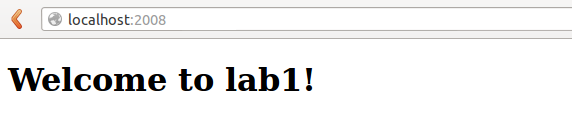
\includegraphics[width=0.4\textwidth]{./imgs/image1.png}
  }
  \caption{Homepage auf 192.168.20.100:8000}
  \label{fig:image1}
\end{figure}
\\
Um herauszufinden um welche Version des Tomcat Server sich handelt, genügt es eine ungültigen Anfrage zum Webserver zu senden. Wenn man z.B. die Resource /wrong auffordert (unter http://localhost:2008/wrong), bekommt man eine Fehlermeldung und man erkennt leicht, dass es sich um einen Tomcat Server Version 6.0.16 handelt.
(\hyperref[fig:image2]{siehe Abbildung~\ref*{fig:image2} auf Seite~\pageref*{fig:image2}}).
\begin{figure}[h!]
  \centering
  \fbox{
    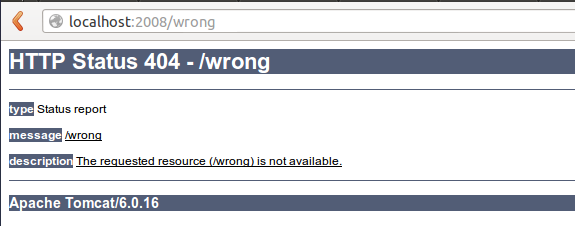
\includegraphics[width=0.4\textwidth]{./imgs/image2.png}
  }
  \caption{Tomcat Version}
  \label{fig:image2}
\end{figure}
\\
Um den privaten Schl"ussel f"ur Benutzer walter zu bekommen, haben wir folgenden Befehl ausgef"uhrt (siehe Schwachstellen und Angriff): \\\url{http://127.0.0.1:2008/\%c0\%ae\%c0\%ae/\%c0\%ae\%c0\%ae/\%c0\%ae\%c0\%ae/\%c0\%ae\%c0\%ae/\%c0\%ae\%c0\%ae/home/walter/.ssh/id_rsa}
\\Mit diesem Schlüssel haben wir einen SSH-Zugang auf dem Server.

\subsection{Schwachstellen und Angriff}
Unter \url{http://tomcat.apache.org/security-6.html} gibt es eine Liste der Tomcat-6.X.X Schwachstellen. Eine Liste der bekannten Schwachstellen für Tomcat-6.0.16 ist unter \\ \url{http://www.cvedetails.com/vulnerability-list/vendor_id-45/product_id-887/version_id-56605/Apache-Tomcat-6.0.16.html} zu finden. Die einzige hier gelistete Schwachstelle, die es einem als Angreifer ermöglicht beliebige Dateien zu lesen, ist Remote UTF-8 Directory Traversal. Eine genaue Beschreibung und Spezifikation findet man unter \url{http://cve.mitre.org/cgi-bin/cvename.cgi?name=CVE-2008-2938}. \\ 
Dieses Problem tritt auf, wenn ``allowLinking'' und ``URIencoding=UTF-8'' im Tomcat erlaubt sind. Der Grund dafür ist, dass JVM UTF-8-kodierte URLs nicht korrekt dekodiert. Wenn das webroot Verzeichnis zB. die Tiefe 3 hat (z.B. /usr/local/wwwroot), kann man auf folgende Weise auf beliebige Daten zugreifen: \\ http://www.target.com/\%c0\%ae\%c0\%ae/\%c0\%ae\%c0\%ae/\%c0\%ae\%c0\%ae/foo/bar   \\Eine mögliche Lösung um solche Angriffe zu vermeiden wäre entweder \"allowLinking\" zu deaktivieren oder \"URIencoding\" nicht auf UTF-8 zu setzen. Noch besser wäre ein Upgrade auf eine neuere Version des Tomcat Server. In der Version 6.0.18 wurde dieses Problem behoben. 


\section{Lab1b}

\subsection{Vorgehensweise}
Nach der Herstellung der SSH-Verbindung wurden zun"achst die lokalen Netzverbindungen mit \texttt{ip addr} ermittelt, wozu auch die IPv6-Adresse mitsamt dem Netzpr"afix geh"orte. Die daraus ersichtlichen Subnetze wurden dann mit \texttt{nmap -sP <subnet>} auf aktive Hosts untersucht, wobei jeder Host anschließend mit \texttt{nmap -sV <host>} auf offene Ports untersucht und der Hostname ermittelt wurde.

Die MAC-Adresse der direkt im selben Subnet befindlichen Hosts konnte aus dem ARP-Cahce mittels \texttt{ip neighbor} ermittelt werden.

Anschließend wurden die angegebenen Subnetze ebenfalls gescannt, wobei die Netztopologie mittels \texttt{traceroute <host>} zu allen Hosts, die in "uber Router erreichbaren Subnetzen lagen, ermittelt. Hierbei fielen einige Inkonsistenzen auf, die im Netzwerkplan dargestellt werden - obwohl Hosts laut ihrer IP-Adresse in einem bestimmten Subnet liegen sollten, welches nur "uber eine Zwischenstation erreichbar war, lieferte \texttt{traceroute} eine direkte Verbindung bzw. eine Verbindung "uber weniger Zwischenstationen als erwartet - daf"ur konnte keine Erkl"arung gefunden werden.

Zum Scan der IPv6-Bereiche wurde ein kleines Skript verwendet, welches "uber die m"oglichen Adressen iterierte und diese \texttt{nmap} zum scan "ubertrug - sp"atere Versionen von \texttt{nmap} k"onnen aber bereits IPv6-Bereiche scannen.

Als Erkl"arung f"ür unterschiedliche Antwortzeiten k"onnte sowohl eine "Uberlastung des einzelnen Hosts, als auch eine Anbindung per VPN in das lokale Netz herangezogen werden, wodurch dann durch die erh"ohte Umlaufzeit Verz"ogerungen auftreten k"onnen.

\subsection{Gefundene Systeme}
Im Bereich 10.12.0.0/24 wurden keine erreichbaren Hosts gefunden.\\
\\
IPv4 Adresse: 192.168.20.254\\
MAC Adresse: 00:e2:aa:21:c5:d1\\
DNS Hostname: Keiner gefunden\\
Offene Ports und Services:\\
Port: 22/tcp, Service: ssh, Version: OpenSSH 5.5p1 Debian 6+squeeze1 (protocol 2.0)\\
Port: 873/tcp, Service: rsync?\\
Installiertes Betriebssystem: Debian Squeeze\\
Vermutete Funktionalit"at: Rsync Server\\
\\
IPv4 Adresse: 192.168.98.1\\
IPv6 Adresse: fdcb:c447:e9d2:3553:1001::1\\
MAC Adresse: 00:1b:d2:0d:84:98\\
DNS Hostname: omega.local.vienna.essecorp.invalid\\
Offene Ports und Services: Alle Ports geschlossen
\\
Installiertes Betriebssystem: Es kann keine Aussage getroffen werden\\
Vermutete Funktionalit"at: Es kann keine Aussage getroffen werden\\
\\
IPv4 Adresse: 192.168.98.10\\
IPv6 Adresse: fdcb:c447:e9d2:3553:1001::5\\
MAC Adresse: 00:1b:d2:d1:1f:85\\
DNS Hostname: alpha.local.vienna.essecorp.invalid\\
Offene Ports und Services:\\
Port: 53/tcp, Service: domain, Version: dnsmasq 2.55\\
Installiertes Betriebssystem: Unix ("ahnlich)\\
Vermutete Funktionalit"at: DNS Server\\
\\
IPv4 Adresse: 192.168.98.28\\
IPv6 Adresse: fdcb:c447:e9d2:3553:1001::9\\
MAC Adresse: 00:1b:d2:f0:60:59\\
DNS Hostname: beta.local.vienna.essecorp.invalid\\
Offene Ports und Services:\\
Port: 25/tcp, Service: smtp?\\
Installiertes Betriebssystem: Es kann keine Aussage getroffen werden, da smtp in verschiedenen Betriebssystemen installierbar ist\\
Vermutete Funktionalit"at: SMTP Server\\
\\
IPv4 Adresse: 192.168.98.54\\
IPv6 Adresse: fdcb:c447:e9d2:3553:1001::21\\
MAC Adresse: 00:1b:d2:83:b8:41\\
DNS Hostname: gamma.local.vienna.essecorp.invalid\\
Offene Ports und Services:\\
Port: 1080/tcp, Service: socks5\\
Installiertes Betriebssystem: Es kann keine Aussage getroffen werden, da socks5 in verschiedenen Betriebssystemen installierbar ist\\
Vermutete Funktionalit"at: Proxy Server\\
\\
IPv4 Adresse: 192.168.98.99\\
IPv6 Adresse: fdcb:c447:e9d2:3553:1001::43\\
MAC Adresse: 00:1b:d2:a7:8f:d2\\
DNS Hostname: delta.local.vienna.essecorp.invalid\\
Offene Ports und Services:\\
Port: 631/tcp, Service: ipp, Version: CUPS 1.4\\
Installiertes Betriebssystem: Es kann keine Aussage getroffen werden, da CUPS in verschiedenen Betriebssystemen installierbar ist\\
Vermutete Funktionalit"at: Print Server\\
\\
Uplink 1:
IPv4 Adresse: 192.168.98.124\\
IPv6 Adresse: fdcb:c447:e9d2:3553:1001::ab\\
MAC Adresse: 00:1b:d7:12:bc:52\\
DNS Hostname: tomcat.local.vienna.essecorp.invalid\\
Uplink 2:
IPv4 Adresse: 192.168.20.100\\
MAC Adresse: 00:1b:d7:12:bc:51\\
Offene Ports und Services:\\
Port: 22/tcp, Service: ssh, Version: OpenSSH 5.5p1 Debian 6+squeeze3 (protocol 2.0)\\
Port: 8000/tcp, Service: http, Version: Apache Tomcat/Coyote JSP engine 1.1\\
Port: 8009/tcp, Service: ajp13\\
Installiertes Betriebssystem: Debian Squeeze\\
Vermutete Funktionalit"at: Web Server\\
\\
IPv4 Adresse: 192.168.98.201\\
IPv6 Adresse: fdcb:c447:e9d2:3553:1001::79\\
MAC Adresse: 00:1b:d2:38:ae:b9\\
DNS Hostname: epsilon.local.vienna.essecorp.invalid\\
Offene Ports und Services:\\
Port: 139/tcp, Service: netbios-ssn, Version: Samba smbd 3.X (workgroup: ESSECORP)\\
Port: 445/tcp, Service: netbios-ssn, Version: Samba smbd 3.X (workgroup: ESSECORP)\\
Installiertes Betriebssystem: Es kann keine Aussage getroffen werden, da samba in verschiedenen Betriebssystemen installierbar ist\\
Vermutete Funktionalit"at:\\
Port 139: NetBIOS Session Service\\
Port 445: Microsoft-DS Active Directory, Windows Shares, Microsoft-DS SMB File Sharing
\\
IPv4 Adresse: 192.168.98.202\\
IPv6 Adresse: fdcb:c447:e9d2:3553:1001::88\\
MAC Adresse: 00:1b:d2:85:9c:c4\\
DNS Hostname: zeta.local.vienna.essecorp.invalid\\
Offene Ports und Services: Alle Ports geschlossen\\
Installiertes Betriebssystem: Es kann keine Aussage getroffen werden\\
Vermutete Funktionalit"at: Es kann keine Aussage getroffen werden\\
\\
IPv4 Adresse: 172.16.2.12\\
MAC Adresse: Keine gefunden\\
DNS Hostname: gemini.dmz.vienna.essecorp.invalid\\
Offene Ports und Services:\\
Port: 80/tcp, Service: http, Version: lighttpd 1.4.28\\
Installiertes Betriebssystem: Es kann keine Aussage getroffen werden, da lighttpd in verschiedenen Betriebssystemen installierbar ist\\
Vermutete Funktionalit"at: Web Server\\
\\
IPv4 Adresse: 172.16.2.15\\
MAC Adresse: Keine gefunden\\
DNS Hostname: phoenix.dmz.vienna.essecorp.invalid\\
Offene Ports und Services:\\
Port: 21/tcp, Service: ftp, Version: vsftpd 2.3.2\\
Installiertes Betriebssystem: Unix ("ahnlich)\\
Vermutete Funktionalit"at: File Server\\
\\
IPv4 Adresse: 172.16.2.25\\
MAC Adresse: Keine gefunden\\
DNS Hostname: taurus.dmz.vienna.essecorp.invalid\\
Offene Ports und Services:\\
Port: 25/tcp, Service: smtp?\\
Installiertes Betriebssystem: Es kann keine Aussage getroffen werden, da smtp in verschiedenen Betriebssystemen installierbar ist\\
Vermutete Funktionalit"at: SMTP Server\\
\\
IPv4 Adresse: 172.16.2.253\\
MAC Adresse: Keine gefunden\\
DNS Hostname: lyra.dmz.vienna.essecorp.invalid\\
Offene Ports und Services: Alle Ports geschlossen\\
Installiertes Betriebssystem: Es kann keine Aussage getroffen werden\\
Vermutete Funktionalit"at: Es kann keine Aussage getroffen werden\\
\\
IPv6 Adresse: fdcb:c447:e9d2:3553:1003::7f\\
MAC Adresse: Keine gefunden\\
DNS Hostname: athena.extra.atlanta.essecorp.invalid\\
Offene Ports und Services:\\
Port: 80/tcp, Service: http, Version: lighttpd 1.4.28\\
Port: 443/tcp, Service: ssl/http, Version: lighttpd 1.4.28\\
Installiertes Betriebssystem: Es kann keine Aussage getroffen werden, da lighttpd in verschiedenen Betriebssystemen installierbar ist\\
Vermutete Funktionalit"at: Web Server (HTTPS)\\
\\
IPv6 Adresse: fdcb:c447:e9d2:3553:1003::9a\\
MAC Adresse: Keine gefunden\\
DNS Hostname: zeus.extra.atlanta.essecorp.invalid\\
Offene Ports und Services:\\
Port: 7/tcp, Service: echo\\
Port: 9/tcp, Service: discard?\\
Port: 13/tcp, Service: daytime\\
Port: 19/tcp, Service: chargen, Version: Linux chargen\\
Port: 22/tcp, Service: ssh, Version: OpenSSH 5.5p1 Debian 6+squeeze3 (protocol 2.0)\\
Port: 37/tcp, Service: time?
Installiertes Betriebssystem: Debian Squeeze\\
Vermutete Funktionalit"at: Es kann keine Aussage getroffen werden\\
\\
IPv6 Adresse: fdcb:c447:e9d2:3553:1003::da\\
MAC Adresse: Keine gefunden\\
DNS Hostname: kerberos.extra.atlanta.essecorp.invalid\\
Offene Ports und Services: Alle Ports geschlossen\\
Installiertes Betriebssystem: Es kann keine Aussage getroffen werden\\
Vermutete Funktionalit"at: Es kann keine Aussage getroffen werden\\
\\
IPv6 Adresse: fdcb:c447:e9d2:3553:1002::fe\\
MAC Adresse: Keine gefunden\\
DNS Hostname: kerberos.dmz.vienna.essecorp.invalid\\
Offene Ports und Services: Alle Ports geschlossen\\
Installiertes Betriebssystem: Es kann keine Aussage getroffen werden\\
Vermutete Funktionalit"at: Es kann keine Aussage getroffen werden\\

\subsection{Netzwerkplan}
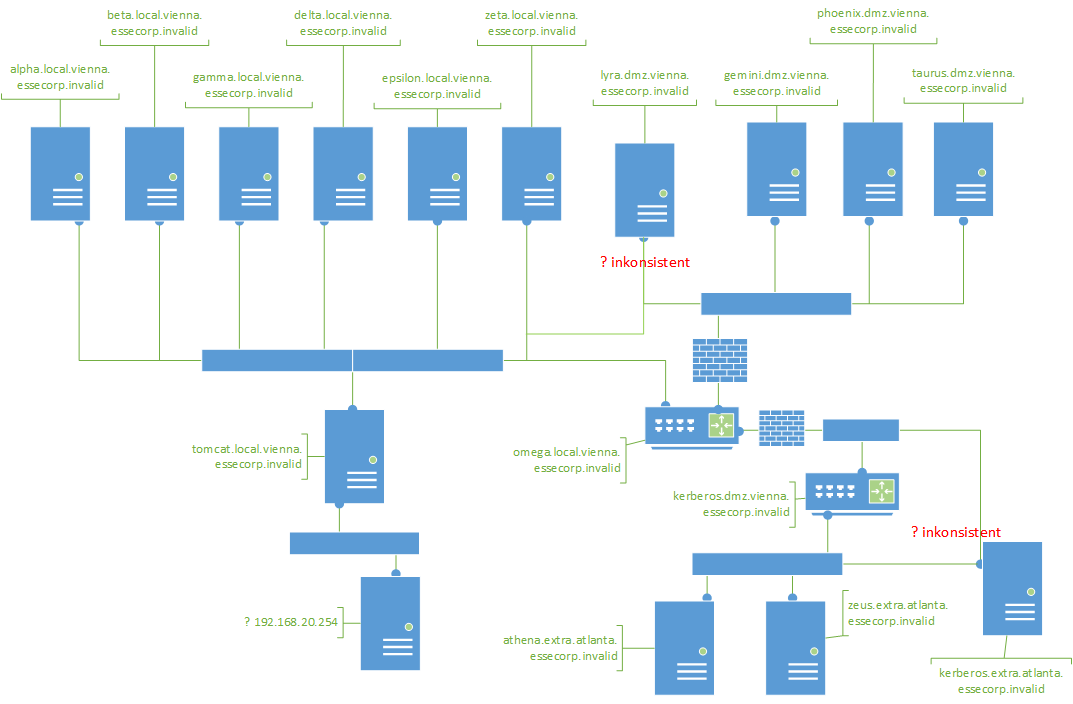
\includegraphics[width=\textwidth]{./imgs/netzwerkplan.png}

\section{Lab1c} 
\subsection{Lab1c - app0}
Im App0 wurden folgende Vulnerabilities gefunden:
\begin{description}
  \item[Integer und Heap-Buffer-Overflow] \hfill \\
  	 Ein Integer-Overflow ist das Ergebnis einer Operation (Addition, Subtraktion, ...), bei der der Wertebereich der Variable überschritten wird.\newline
  	 Ein Heap-Buffer-Overflow bezeichnet den Zugriff außerhalb der Grenzen des allozierten Speichers. Beispielsweise:
  	 \begin{lstlisting}
var=malloc(10);
var[11]=5;
	\end{lstlisting}
	Dabei ist es möglich, Funktionspointer oder andere wichtige Datenstrukturen am Heap eines Programmes zu überschreiben um dadurch entweder die Kontrolle zu übernehmen, oder das Programm zum absturz zu bringen.\newline
	
  	 Beispielsweise wird in app0 -1 von einem size\_t-Typ mit dem Wert 0 (Ergebnis der strlen-Funktion) subtrahiert. Da size\_t unsigned ist, f"uhrt das zu einem wrap-around, so dass der neue Wert 0xFFFFFFFFFFFFFFFF ist. \newline
    Dieser Bug f"uhrt in weiter folge zu einem Heap-Buffer-Overflow, da i weit "uber MAX wachsen kann.\newline
    Diese beiden Overflows befinden sich in der Funktion strip (Zeile 12). Sie lassen sich durch eine leere Eingabe ausl"osen (da strlen dann 0 zur"uckliefert).\newline
    Vorgehensweise:
    \begin{itemize}
    \item Eine leere Eingabe machen (,,Enter'' dr"ucken)
    \end {itemize}
    Diese Vulnerability kann in dem Fall f"ur ein DOS genutzt werden.\\
    Diese Vulnerability wird mit dem Script ,,heap\_int\_overflow.sh'' ausgenutzt.\\
    \\
    Eine Heap Overflow Schwachstelle wurde in Oracle Java JRE \& JDK 7u7 und vorherigen Versionen gefunden. Die Schwachstelle befindet sich in ``t2k.dll'', genauer in ``maxCountPoint'' eines Fonts, und k"onnte von einem Angreifer durch eine spezielle Webseite ausgen"utzt werden. Diese Schwachstelle ist kritisch und hat den h"ochsten CVSS Score, n"amlich 10.\newline
    Quelle: \url{http://seclists.org/bugtraq/2012/Oct/119}
    
  \item[Format-String] \hfill \\
  Funktionen der printf-Familie verwenden Format-Strings zur Steuerungs ihres verhaltens. Werden dabei spezielle Sequenzen, wie z.B. \%u, \%s oder \%n vorgefunden, so nimmt der Code an, dass entsprechende Argumente "ubergeben worden sind (und daher am Stack liegen). Ist nun der Format-String vom Benutzer beeinflussbar, so kann dadurch ein nicht vorhergesehenes Verhalten der Funktionen ausgel"ost, und damit der Programmablauf ver"andert werden.\newline
  In der Funktion outprint (main.c:56, main.c:60) wird der vom User eingegebene String als Format-String an printf "ubergeben.\newline
  Vorgehensweise (DOS/PoC):
  \begin{itemize}
  \item Den String ,,\%100\$s'' "uberpr"ufen lassen (ohne Anf"uhrungszeichen eingeben)
  \end{itemize}
  Da das Program nun wahrscheinlich abst"urzt (eventuell muss der Parameter 100 ge"andert werden), kann man davon ausgehen, dass eine Format-String-Vulnerability vorliegt (der String sollte nicht lang genug f"ur einen Buffer-Overflow sein).\newline
  Durch die \%s und \%n Sequenz ist es m"oglich, an beliebige Stellen im Speicher zu lesen bzw. schreiben.\newline
    Um diese Vulnerability zum Ausf"uhren vom Shellcode nutzen zu k"onnen, sind folgende Schritte notwendig:
    \begin{itemize}
        \item Format-Offset bestimmen (=,,Wie viele Bytes m"ussen vom Stack gepopt werden, bevor der der Input-Buffer erreicht wird'')
        \item Zur CPU-Archtektur passenden Format-Offset zum oberem addieren, um die Adresse einer Stack-Frame zu erhalten.
        \item Aus dem Frame-Pointer, durch die CPU-Archektur und Compiler bestimmt, den Offset f"ur den Return-Pointer auf dem Stack bestimmen.
        \item Durch den Format-Offset und den Stack-Frame-Pointer l"asst sich die Adresse des input-Buffers bestimmen.
        \item Aus diesen Daten kann der String für den Angriff generiert werden:\\
        \begin{lstlisting}
${ripAdresse}$(($inputBufferAdresse-2*$Adresslaenge+$offsetZumShellCode))%${formatOffset}\$n${shellCode}
        \end{lstlisting}
    \end{itemize}
    Anm.: Dieser Angriff funkioniert auch auf Systemen mit ASLR. Der obere String ist in einer bash-"ahnlichen Syntax.\newline
    Der geschriebene Wert befindet sich im zweiten Teil des Strings. Ohne Shellcode, kann man dadurch einen Wert auf eine Adresse schreiben.\newline
    Beispielsweise schreibt der String
    \begin{lstlisting}
aaaaaaaa%992u%18$n
	 \end{lstlisting}
	 den Wert 1000 an die Adresse 0x6161616161616161.\newline
    Diese Vulnerability wird durch das Skript ,,format\_string.sh'' ausgenutzt. Dabei kann man eine Addresse und einen Wert angeben, der dorthin geschrieben werden soll.\newline
    Da der Input-Buffer nur 41 Byte groß ist, werden in ,,format\_string.sh'' die Escape-Sequenzen nicht direkt im String gehalten, sondern bereits evaluiert, so dass nicht-ASCII-Zeichen an das Program "ubergeben werden m"ussen.
    
    Format-String-Vulnerabilities wurden beispielsweise im Exim Daemon, im Linux Kernel und im Windows Printer Spooler gefunden. Vor allem die Windows Printer Spooler ist sehr gef"ahrlich, da dieser Dienst in der Standardkonfiguration von Windows-System aktiv ist.
    Quellen:
    \begin{itemize}
    \item \url{http://web.nvd.nist.gov/view/vuln/detail?vulnId=CVE-2012-1851}
    \item \url{http://web.nvd.nist.gov/view/vuln/detail?vulnId=CVE-2011-1764}
    \item \url{https://web.nvd.nist.gov/view/vuln/detail?vulnId=CVE-2013-1848}
\end{itemize}
    \item[Memory Leak]
    Ein Memory-Leak ist ein Speicherbereich auf den das Programm keinen Zugriff mehr hat. Memory-Leaks können beispielsweise dadurch entstehen, dass Pointer auf allozierten Speicher "uberschrieben werden.
    Da der in strip allozierte Speicher (main.c:15) nie freigegeben wird, wird ab einem Zeitpunkt kein freier Speicher am Heap zur Verfügung stehen. Da malloc in diesem Fall meist NULL liefert, wird das Programm, beim Versuch diese Adresse zu benutzen (main.c:18), terminiert (DOS-Angriff).\newline
    
Vorgehensweise:
\begin{itemize}
	\item Dem Programm wiederholend (viele Wiederholungen notwendig) neue Strings eingeben.
\end{itemize}
Anm.: es empfiehlt sich, eine Schleife zu verwenden. Siehe memory\_leak.sh.\newline
    
    Im SNMP Module des Cisco IOS XR wurde eine Schwachstelle entdeckt, die es einem Angreifer erm"oglicht durch speziell angefertige SNMP Packete einen Memory Leak auszul"osen. Die Schwachstelle entsteht dadurch, dass der Input nicht genug "Uberpr"uft wird. Der SNMP Prozess startet neu, sobald der ihm zugeteilte Speicher voll ist. Diese Schwachstelle wurde als eher gering gef"ahrlich eingestuft.\newline
    Quelle: \url{http://tools.cisco.com/security/center/content/CiscoSecurityNotice/CVE-2013-1216}
\end{description}

\subsection{Lab1c - app1}
Beim Cross-Site-Scripting (XSS) wird in eine bestehende Seite ein Javascript-Code injiziert, wenn die Eingabefelder nicht serverseitig richtig validiert werden.\newline
Es gibt Stored- und Reflected-XSS.
Beispielseingabe: <script type="text/javascript">alert("Das ist XSS");</script>.

Im Beispiel app2 wird zwar die Benutzereingabe validiert, jedoch nur ungen"ugend (siehe ScriptTagValidator.java:9).

Triggern:
Vorraussetzung: Laufende Web-Applikation, Bekannte IP-Adresse und Port der Web-Applikation.

Vorgehensweise:
\begin{itemize}
	\item Seite "offnen um das Session-Cookie zu bekommen
	\item Einen POST-HTTP-Request an /blog/post mit dem Inhalt ``author=\$beliebig\&content=\$scriptCode'' und dem vorher erwähntem Cookie schicken.
\end{itemize}

Nun wird bei jedem Benutzer, der diesen Post sieht, ein JS-Code ausgef"uhrt welcher vom (vertauensw"urdigen) Server zu kommen scheint.

Anmerkung: Diese Vulnerability l"asst sich grunds"atzlich auch nutzen um beliebigen XHTML-Code einzuf"ugen.

\subsection{Lab1c - app2}

In app2 wurde eine \textit{weak session id}-L"ucke gefunden, die es einem Angreifer erlauben w"urde, die aktuelle Session-ID eines angemeldeten Nutzers zu erraten bzw. errechnen und an den Server zu senden. Dieser nimmt nun an, mit den tatsächlichen Nutzer zu kommunizieren, da die ID als Geheimnis nur zwischen Server und Nutzer bekannt sein sollte, eine weitere Authentifizierung (z.B. anhand der IP-Adresse) findet nicht statt.

Die Lücke ist in der Datei \texttt{src/functions.php} innerhalb der Funktion \texttt{make\_new\_session()}, in der die Session-ID auf folgende Weise erzeugt wird (Zeile 87): \lstinline{$sessionid = md5($time."|".$this->data["username"]);}

Die Applikation erzeugt aus der aktuellen Unix-Zeit des Servers verkettet mit dem Nutzernamen einen MD5-Hash, der anschließend als Session-ID verwendet wird. Sowohl Server-Zeit als auch Benutzernamen werden allen Besuchern der Applikation auf der Hauptseite angezeigt - ein Angreifer muss nur die Unix-Zeit bei der Anmeldung des Ziel-Benutzers erraten, in dem von der aktuellen Zeit der Wert in Minuten seit der letzten Anmeldung subtrahiert wird (auch diese Information wird unn"otigerweise allen Besuchern gezeigt). Durch Ausprobieren verschiedener Verkettungs-Zeichen, Reihenfolgen und anschließendem Hashing kann der Angreifer letztendlich an die Session ID gelangen und hat Zugriff auf das Profil des Benutzers ohne dass ein Passwort etc. notwendig ist - selbst die Verschlüsselung der Kommunikation zwischen Benutzer und Server ist bei dieser Art des Angriffs wirkungslos.

Konkret müssen also folgende Schritte durchgeführt werden, um die Session eines Nutzers zu kapern:

\begin{itemize}
\item Aufruf der Hauptseite und Extraktion eines Benutzernamens, der verstrichenen Zeit seit der dessen Anmeldung und die Serverzeit
\item Rückrechnen der Systemzeit bei der Anmeldung des Benutzers, wobei eine gewisse Toleranz ber"ucksichtigt wird
\item Schrittweise Erzeugung einer Session-ID durch iterative Auswahl einer Systemzeit aus dem Toleranzintervall verkettet mit \texttt{|} und dem Benutzernamen, sowie anschließendem Hashing mit MD5.
\item Die erzeugte Session-ID wird dem Server innerhalb einer Anfrage übermittelt - ist sie ung"ultig, erh"alt der Angreifer nur eine Gast-Seite, bei Akzeptanz durch den Server wird die benutzer-spezifische Seite "ubermittelt und der Angriff war erfolgreich.
\end{itemize}

Um den Fehler zu beheben, kann statt der durch die Applikation selbst implementierten Session-Mechanik auf die als resistent geltenden Implementierungen des Frameworks bzw. der Sprache zur"uckgegriffen werden, in Beispiel von PHP etwa durch die Funktionen \texttt{session\_start}, \texttt{session\_id} etc. Stattdessen kann die Erzeugung der Session-ID auch abgesichert werden, indem die Informationen, die in die Erzeugung einfließen, nur dem betreffenden Nutzer selbst angezeigt werden oder zuf"allige Faktoren einfließen, die ein Angreifer nicht in realistischer Weise erraten kann - beispielsweise durch den Server generierte Pseudozufallszahlen kombiniert mit der Serverzeit. 

In unserer korrigierten Version wird zur Erzeugung der Session-ID ausschließlich eine Zufallszahl verwendet, die anschließend wieder verworfen wird: \lstinline{$sessionid = md5(rand());} Ein Angreifer hat keine M"oglichkeit, von außen an die Zufallszahl zu gelangen und der hohe m"ogliche Wertebereich verhindert ein Erraten der Zahl durch simples Ausprobieren. Zu beachten bei der Verwendung von Pseudo-Zufallszahlen ist eine m"oglichst hohe Entropie bei der Wahl des Initialisierungswertes, da sich s"amtliche erzeugte Zufallszahlen berechnen lassen, wenn ein Angreifer diesen Wert erraten kann.

Es wurde neben anderen kritischen Schwachstellen auch eine kritische Weak Session ID Schwachstelle in Cisco Unified Videoconferencing 3515,3522,3527,5230,3545,5110,5115 Systemen gefunden. Session IDs sind auf diesen Systemen die Timestamps zu denen sich die Benutzer eingeloggt haben und sind trivial nachzubauen. Diese Timestamps herauszufinden ist z.B. "uber RPC m"oglich. Durch diese Schwachstelle kann sich ein unauthentifizierter Angreifer am System authentifizieren.\newline
Quelle: \url{http://seclists.org/fulldisclosure/2010/Nov/167}

\section{Beispiele}

\subsection{Source Code formatieren}
Es folgen einige Beispiele wie Sourcecode in diesem Dokument formatiert und referenziert werden kann
(\hyperref[code:beispiel1]{siehe Listing~\ref*{code:beispiel1} auf Seite~\pageref*{code:beispiel1}} und \hyperref[code:beispiel2]{siehe Listing~\ref*{code:beispiel2} auf Seite~\pageref*{code:beispiel2}}).

Ebenso k"onnen kurzer Code oder kurze Befehle direkt in der Zeile in einem \lstinline{lstinline Block} mit typengleicher Schrift formatiert werden.

%\lstinputlisting[caption=Example C/C++ file,label=code:beispiel1,style=c]{example.c}

\begin{lstlisting}[caption=Example bash script,label=code:beispiel2,style=simple]
#!/bin/bash
echo "Bash version ${BASH_VERSION}..."
for i in {0..10..2}
  do
     echo ``Welcome $i times''
 done

echo ``some very very very very very very very very very very very very very very very very very very very very long string''s

exit 0;
\end{lstlisting}

\subsection{Bilder}

Es folgen einige Beispiele wie Bilder in diesem Dokument eingefuegt werden koennen
(\hyperref[fig:logo1]{siehe Abbildung~\ref*{fig:logo1} auf Seite~\pageref*{fig:logo1}}).

\begin{figure}[h!]
  \centering
  \fbox{
    
\includegraphics[width=0.4\textwidth]{./imgs/esse-logo-bw.png}
  }
  \caption{ESSE Logo}
  \label{fig:logo1}
\end{figure}


\end{document}


